\documentclass[1p]{elsarticle_modified}
%\bibliographystyle{elsarticle-num}

%\usepackage[colorlinks]{hyperref}
%\usepackage{abbrmath_seonhwa} %\Abb, \Ascr, \Acal ,\Abf, \Afrak
\usepackage{amsfonts}
\usepackage{amssymb}
\usepackage{amsmath}
\usepackage{amsthm}
\usepackage{scalefnt}
\usepackage{amsbsy}
\usepackage{kotex}
\usepackage{caption}
\usepackage{subfig}
\usepackage{color}
\usepackage{graphicx}
\usepackage{xcolor} %% white, black, red, green, blue, cyan, magenta, yellow
\usepackage{float}
\usepackage{setspace}
\usepackage{hyperref}

\usepackage{tikz}
\usetikzlibrary{arrows}

\usepackage{multirow}
\usepackage{array} % fixed length table
\usepackage{hhline}

%%%%%%%%%%%%%%%%%%%%%
\makeatletter
\renewcommand*\env@matrix[1][\arraystretch]{%
	\edef\arraystretch{#1}%
	\hskip -\arraycolsep
	\let\@ifnextchar\new@ifnextchar
	\array{*\c@MaxMatrixCols c}}
\makeatother %https://tex.stackexchange.com/questions/14071/how-can-i-increase-the-line-spacing-in-a-matrix
%%%%%%%%%%%%%%%

\usepackage[normalem]{ulem}

\newcommand{\msout}[1]{\ifmmode\text{\sout{\ensuremath{#1}}}\else\sout{#1}\fi}
%SOURCE: \msout is \stkout macro in https://tex.stackexchange.com/questions/20609/strikeout-in-math-mode

\newcommand{\cancel}[1]{
	\ifmmode
	{\color{red}\msout{#1}}
	\else
	{\color{red}\sout{#1}}
	\fi
}

\newcommand{\add}[1]{
	{\color{blue}\uwave{#1}}
}

\newcommand{\replace}[2]{
	\ifmmode
	{\color{red}\msout{#1}}{\color{blue}\uwave{#2}}
	\else
	{\color{red}\sout{#1}}{\color{blue}\uwave{#2}}
	\fi
}

\newcommand{\Sol}{\mathcal{S}} %segment
\newcommand{\D}{D} %diagram
\newcommand{\A}{\mathcal{A}} %arc


%%%%%%%%%%%%%%%%%%%%%%%%%%%%%5 test

\def\sl{\operatorname{\textup{SL}}(2,\Cbb)}
\def\psl{\operatorname{\textup{PSL}}(2,\Cbb)}
\def\quan{\mkern 1mu \triangleright \mkern 1mu}

\theoremstyle{definition}
\newtheorem{thm}{Theorem}[section]
\newtheorem{prop}[thm]{Proposition}
\newtheorem{lem}[thm]{Lemma}
\newtheorem{ques}[thm]{Question}
\newtheorem{cor}[thm]{Corollary}
\newtheorem{defn}[thm]{Definition}
\newtheorem{exam}[thm]{Example}
\newtheorem{rmk}[thm]{Remark}
\newtheorem{alg}[thm]{Algorithm}

\newcommand{\I}{\sqrt{-1}}
\begin{document}

%\begin{frontmatter}
%
%\title{Boundary parabolic representations of knots up to 8 crossings}
%
%%% Group authors per affiliation:
%\author{Yunhi Cho} 
%\address{Department of Mathematics, University of Seoul, Seoul, Korea}
%\ead{yhcho@uos.ac.kr}
%
%
%\author{Seonhwa Kim} %\fnref{s_kim}}
%\address{Center for Geometry and Physics, Institute for Basic Science, Pohang, 37673, Korea}
%\ead{ryeona17@ibs.re.kr}
%
%\author{Hyuk Kim}
%\address{Department of Mathematical Sciences, Seoul National University, Seoul 08826, Korea}
%\ead{hyukkim@snu.ac.kr}
%
%\author{Seokbeom Yoon}
%\address{Department of Mathematical Sciences, Seoul National University, Seoul, 08826,  Korea}
%\ead{sbyoon15@snu.ac.kr}
%
%\begin{abstract}
%We find all boundary parabolic representation of knots up to 8 crossings.
%
%\end{abstract}
%\begin{keyword}
%    \MSC[2010] 57M25 
%\end{keyword}
%
%\end{frontmatter}

%\linenumbers
%\tableofcontents
%
\newcommand\colored[1]{\textcolor{white}{\rule[-0.35ex]{0.8em}{1.4ex}}\kern-0.8em\color{red} #1}%
%\newcommand\colored[1]{\textcolor{white}{ #1}\kern-2.17ex	\textcolor{white}{ #1}\kern-1.81ex	\textcolor{white}{ #1}\kern-2.15ex\color{red}#1	}

{\Large $\underline{12a_{1227}~(K12a_{1227})}$}

\setlength{\tabcolsep}{10pt}
\renewcommand{\arraystretch}{1.6}
\vspace{1cm}\begin{tabular}{m{100pt}>{\centering\arraybackslash}m{274pt}}
\multirow{5}{120pt}{
	\centering
	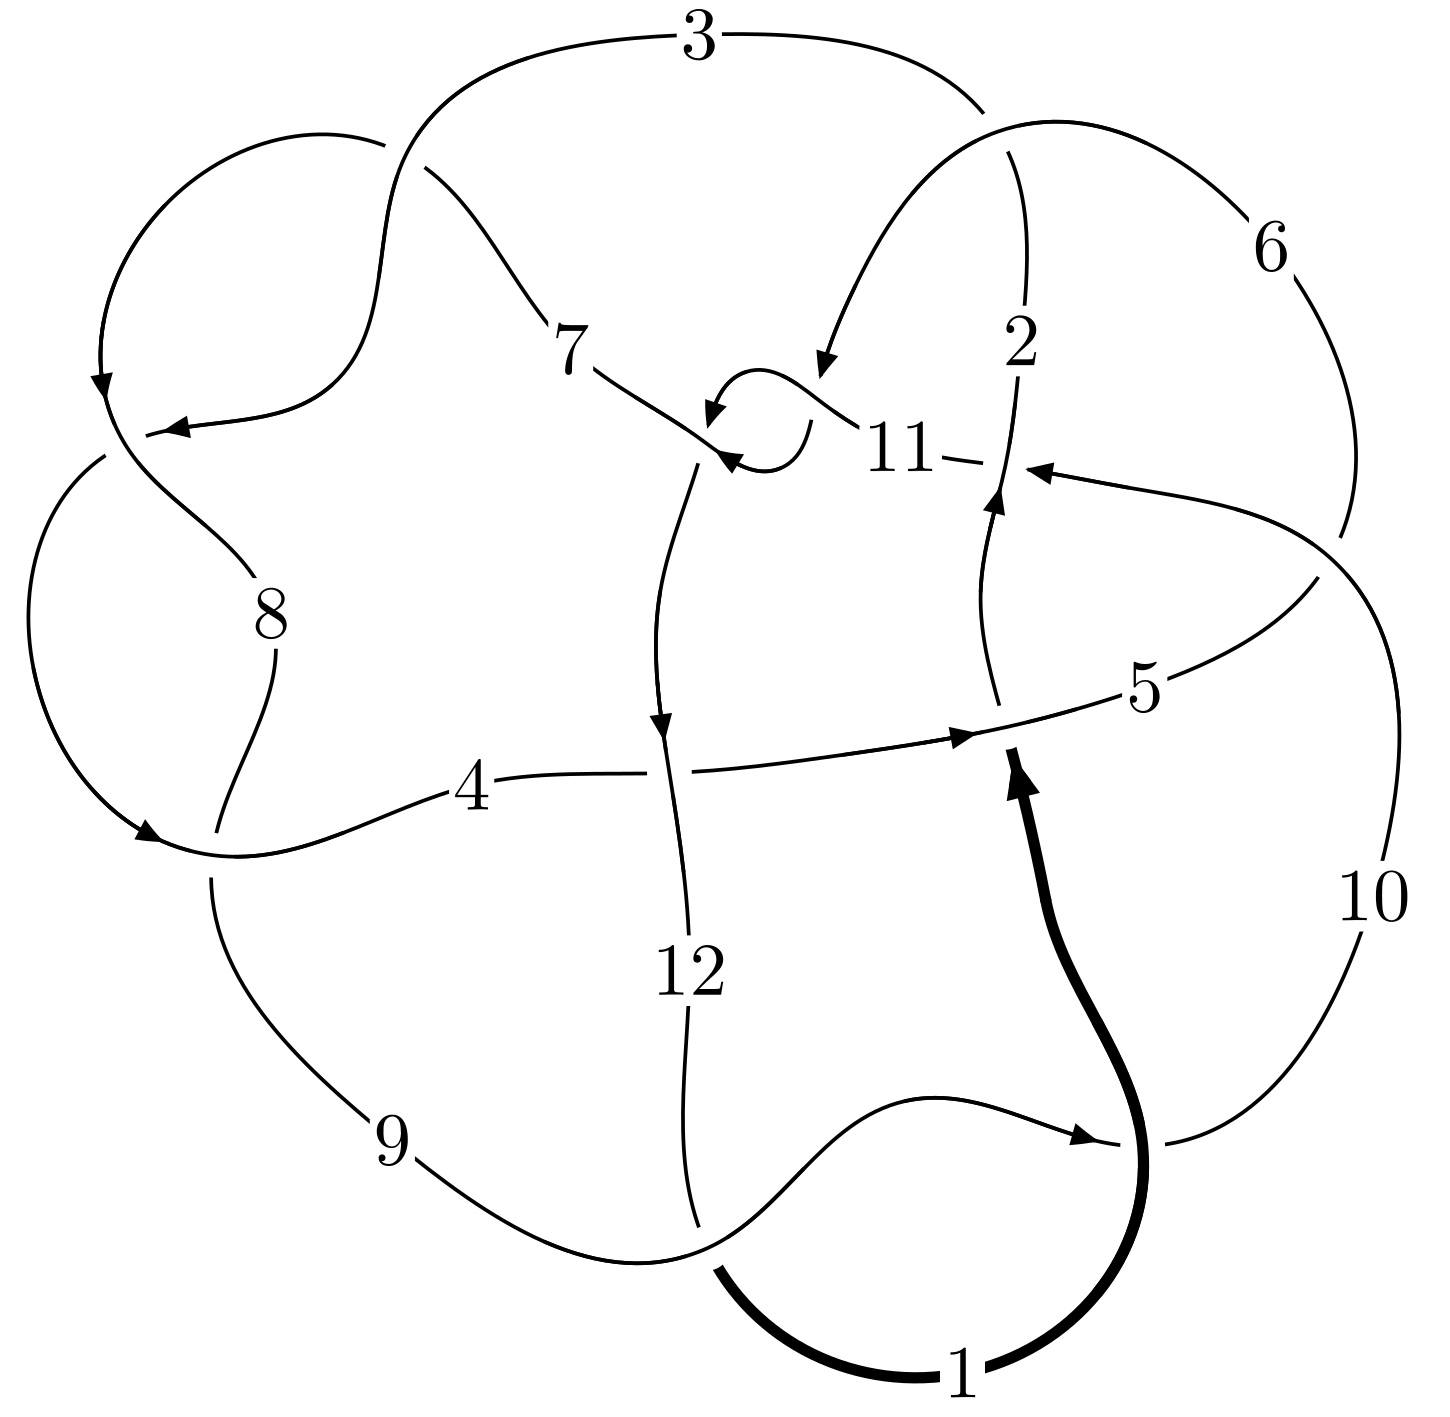
\includegraphics[width=112pt]{../../../GIT/diagram.site/Diagrams/png/2028_12a_1227.png}\\
\ \ \ A knot diagram\footnotemark}&
\allowdisplaybreaks
\textbf{Linearized knot diagam} \\
\cline{2-2}
 &
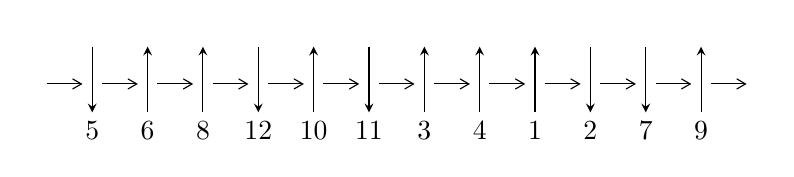
\begin{tikzpicture}[x=20pt, y=17pt]
	% nodes
	\node (C0) at (0, 0) {};
	\node (C1) at (1, 0) {};
	\node (C1U) at (1, +1) {};
	\node (C1D) at (1, -1) {5};

	\node (C2) at (2, 0) {};
	\node (C2U) at (2, +1) {};
	\node (C2D) at (2, -1) {6};

	\node (C3) at (3, 0) {};
	\node (C3U) at (3, +1) {};
	\node (C3D) at (3, -1) {8};

	\node (C4) at (4, 0) {};
	\node (C4U) at (4, +1) {};
	\node (C4D) at (4, -1) {12};

	\node (C5) at (5, 0) {};
	\node (C5U) at (5, +1) {};
	\node (C5D) at (5, -1) {10};

	\node (C6) at (6, 0) {};
	\node (C6U) at (6, +1) {};
	\node (C6D) at (6, -1) {11};

	\node (C7) at (7, 0) {};
	\node (C7U) at (7, +1) {};
	\node (C7D) at (7, -1) {3};

	\node (C8) at (8, 0) {};
	\node (C8U) at (8, +1) {};
	\node (C8D) at (8, -1) {4};

	\node (C9) at (9, 0) {};
	\node (C9U) at (9, +1) {};
	\node (C9D) at (9, -1) {1};

	\node (C10) at (10, 0) {};
	\node (C10U) at (10, +1) {};
	\node (C10D) at (10, -1) {2};

	\node (C11) at (11, 0) {};
	\node (C11U) at (11, +1) {};
	\node (C11D) at (11, -1) {7};

	\node (C12) at (12, 0) {};
	\node (C12U) at (12, +1) {};
	\node (C12D) at (12, -1) {9};
	\node (C13) at (13, 0) {};

	% arrows
	\draw[->,>={angle 60}]
	(C0) edge (C1) (C1) edge (C2) (C2) edge (C3) (C3) edge (C4) (C4) edge (C5) (C5) edge (C6) (C6) edge (C7) (C7) edge (C8) (C8) edge (C9) (C9) edge (C10) (C10) edge (C11) (C11) edge (C12) (C12) edge (C13) ;	\draw[->,>=stealth]
	(C1U) edge (C1D) (C2D) edge (C2U) (C3D) edge (C3U) (C4U) edge (C4D) (C5D) edge (C5U) (C6U) edge (C6D) (C7D) edge (C7U) (C8D) edge (C8U) (C9D) edge (C9U) (C10U) edge (C10D) (C11U) edge (C11D) (C12D) edge (C12U) ;
	\end{tikzpicture} \\
\hhline{~~} \\& 
\textbf{Solving Sequence} \\ \cline{2-2} 
 &
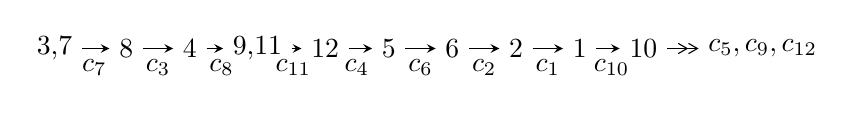
\begin{tikzpicture}[x=23pt, y=7pt]
	% node
	\node (A0) at (-1/8, 0) {3,7};
	\node (A1) at (1, 0) {8};
	\node (A2) at (2, 0) {4};
	\node (A3) at (49/16, 0) {9,11};
	\node (A4) at (33/8, 0) {12};
	\node (A5) at (41/8, 0) {5};
	\node (A6) at (49/8, 0) {6};
	\node (A7) at (57/8, 0) {2};
	\node (A8) at (65/8, 0) {1};
	\node (A9) at (73/8, 0) {10};
	\node (C1) at (1/2, -1) {$c_{7}$};
	\node (C2) at (3/2, -1) {$c_{3}$};
	\node (C3) at (5/2, -1) {$c_{8}$};
	\node (C4) at (29/8, -1) {$c_{11}$};
	\node (C5) at (37/8, -1) {$c_{4}$};
	\node (C6) at (45/8, -1) {$c_{6}$};
	\node (C7) at (53/8, -1) {$c_{2}$};
	\node (C8) at (61/8, -1) {$c_{1}$};
	\node (C9) at (69/8, -1) {$c_{10}$};
	\node (A10) at (11, 0) {$c_{5},c_{9},c_{12}$};

	% edge
	\draw[->,>=stealth]	
	(A0) edge (A1) (A1) edge (A2) (A2) edge (A3) (A3) edge (A4) (A4) edge (A5) (A5) edge (A6) (A6) edge (A7) (A7) edge (A8) (A8) edge (A9) ;
	\draw[->>,>={angle 60}]	
	(A9) edge (A10);
\end{tikzpicture} \\ 

\end{tabular} \\

\footnotetext{
The image of knot diagram is generated by the software ``\textbf{Draw programme}" developed by Andrew Bartholomew(\url{http://www.layer8.co.uk/maths/draw/index.htm\#Running-draw}), where we modified some parts for our purpose(\url{https://github.com/CATsTAILs/LinksPainter}).
}\phantom \\ \newline 
\centering \textbf{Ideals for irreducible components\footnotemark of $X_{\text{par}}$} 
 
\begin{align*}
I^u_{1}&=\langle 
7.98393\times10^{349} u^{118}+1.68479\times10^{350} u^{117}+\cdots+6.11588\times10^{349} b+3.23054\times10^{349},\\
\phantom{I^u_{1}}&\phantom{= \langle  }-1.60699\times10^{350} u^{118}-1.85142\times10^{350} u^{117}+\cdots+6.11588\times10^{349} a+3.45671\times10^{351},\\
\phantom{I^u_{1}}&\phantom{= \langle  }u^{119}+u^{118}+\cdots+24 u-1\rangle \\
I^u_{2}&=\langle 
-357 u^{23}+327 u^{22}+\cdots+1579 b+1708,\;-19392 u^{23}+8169 u^{22}+\cdots+30001 a+14942,\\
\phantom{I^u_{2}}&\phantom{= \langle  }u^{24}-16 u^{22}+\cdots+4 u-1\rangle \\
\\
\end{align*}
\raggedright * 2 irreducible components of $\dim_{\mathbb{C}}=0$, with total 143 representations.\\
\footnotetext{All coefficients of polynomials are rational numbers. But the coefficients are sometimes approximated in decimal forms when there is not enough margin.}
\newpage
\renewcommand{\arraystretch}{1}
\centering \section*{I. $I^u_{1}= \langle 7.98\times10^{349} u^{118}+1.68\times10^{350} u^{117}+\cdots+6.12\times10^{349} b+3.23\times10^{349},\;-1.61\times10^{350} u^{118}-1.85\times10^{350} u^{117}+\cdots+6.12\times10^{349} a+3.46\times10^{351},\;u^{119}+u^{118}+\cdots+24 u-1 \rangle$}
\flushleft \textbf{(i) Arc colorings}\\
\begin{tabular}{m{7pt} m{180pt} m{7pt} m{180pt} }
\flushright $a_{3}=$&$\begin{pmatrix}0\\u\end{pmatrix}$ \\
\flushright $a_{7}=$&$\begin{pmatrix}1\\0\end{pmatrix}$ \\
\flushright $a_{8}=$&$\begin{pmatrix}1\\- u^2\end{pmatrix}$ \\
\flushright $a_{4}=$&$\begin{pmatrix}u\\- u^3+u\end{pmatrix}$ \\
\flushright $a_{9}=$&$\begin{pmatrix}- u^2+1\\u^4-2 u^2\end{pmatrix}$ \\
\flushright $a_{11}=$&$\begin{pmatrix}2.62757 u^{118}+3.02724 u^{117}+\cdots+182.921 u-56.5203\\-1.30544 u^{118}-2.75478 u^{117}+\cdots-32.8072 u-0.528222\end{pmatrix}$ \\
\flushright $a_{12}=$&$\begin{pmatrix}3.93302 u^{118}+5.78201 u^{117}+\cdots+215.728 u-55.9920\\-1.30544 u^{118}-2.75478 u^{117}+\cdots-32.8072 u-0.528222\end{pmatrix}$ \\
\flushright $a_{5}=$&$\begin{pmatrix}-9.05213 u^{118}-12.4473 u^{117}+\cdots-1075.39 u-12.4747\\-2.62416 u^{118}-5.54499 u^{117}+\cdots-122.351 u+2.00968\end{pmatrix}$ \\
\flushright $a_{6}=$&$\begin{pmatrix}3.77228 u^{118}+4.58088 u^{117}+\cdots+16.4140 u-72.6929\\-2.33609 u^{118}-5.29085 u^{117}+\cdots-40.3513 u-1.16876\end{pmatrix}$ \\
\flushright $a_{2}=$&$\begin{pmatrix}-8.43648 u^{118}-4.70064 u^{117}+\cdots-2933.04 u-14.4301\\0.0426533 u^{118}+0.286147 u^{117}+\cdots-84.7869 u-0.871764\end{pmatrix}$ \\
\flushright $a_{1}=$&$\begin{pmatrix}2.96289 u^{118}+3.85385 u^{117}+\cdots+199.978 u-56.9956\\-1.06822 u^{118}-2.22728 u^{117}+\cdots-32.5595 u-0.513198\end{pmatrix}$ \\
\flushright $a_{10}=$&$\begin{pmatrix}-3.11074 u^{118}+1.76443 u^{117}+\cdots-459.746 u+91.1873\\-0.992728 u^{118}-2.77364 u^{117}+\cdots+58.9070 u+0.0751447\end{pmatrix}$\\&\end{tabular}
\flushleft \textbf{(ii) Obstruction class $= -1$}\\~\\
\flushleft \textbf{(iii) Cusp Shapes $= 5.87699 u^{118}+9.13379 u^{117}+\cdots+382.108 u-20.5150$}\\~\\
\newpage\renewcommand{\arraystretch}{1}
\flushleft \textbf{(iv) u-Polynomials at the component}\newline \\
\begin{tabular}{m{50pt}|m{274pt}}
Crossings & \hspace{64pt}u-Polynomials at each crossing \\
\hline $$\begin{aligned}c_{1}\end{aligned}$$&$\begin{aligned}
&u^{119}-6 u^{118}+\cdots-9 u-1
\end{aligned}$\\
\hline $$\begin{aligned}c_{2}\end{aligned}$$&$\begin{aligned}
&u^{119}-6 u^{117}+\cdots-511 u-31
\end{aligned}$\\
\hline $$\begin{aligned}c_{3},c_{7},c_{8}\end{aligned}$$&$\begin{aligned}
&u^{119}+u^{118}+\cdots+24 u-1
\end{aligned}$\\
\hline $$\begin{aligned}c_{4}\end{aligned}$$&$\begin{aligned}
&u^{119}+23 u^{117}+\cdots+67021094 u-10361027
\end{aligned}$\\
\hline $$\begin{aligned}c_{5}\end{aligned}$$&$\begin{aligned}
&u^{119}+3 u^{118}+\cdots+10287 u+923
\end{aligned}$\\
\hline $$\begin{aligned}c_{6},c_{11}\end{aligned}$$&$\begin{aligned}
&u^{119}- u^{118}+\cdots-3875 u+1543
\end{aligned}$\\
\hline $$\begin{aligned}c_{9},c_{12}\end{aligned}$$&$\begin{aligned}
&u^{119}-3 u^{118}+\cdots-75 u+25
\end{aligned}$\\
\hline $$\begin{aligned}c_{10}\end{aligned}$$&$\begin{aligned}
&u^{119}+5 u^{118}+\cdots-11110 u-1273
\end{aligned}$\\
\hline
\end{tabular}\\~\\
\newpage\renewcommand{\arraystretch}{1}
\flushleft \textbf{(v) Riley Polynomials at the component}\newline \\
\begin{tabular}{m{50pt}|m{274pt}}
Crossings & \hspace{64pt}Riley Polynomials at each crossing \\
\hline $$\begin{aligned}c_{1}\end{aligned}$$&$\begin{aligned}
&y^{119}-8 y^{118}+\cdots-343 y-1
\end{aligned}$\\
\hline $$\begin{aligned}c_{2}\end{aligned}$$&$\begin{aligned}
&y^{119}-12 y^{118}+\cdots+125031 y-961
\end{aligned}$\\
\hline $$\begin{aligned}c_{3},c_{7},c_{8}\end{aligned}$$&$\begin{aligned}
&y^{119}-129 y^{118}+\cdots+2056 y-1
\end{aligned}$\\
\hline $$\begin{aligned}c_{4}\end{aligned}$$&$\begin{aligned}
&y^{119}+46 y^{118}+\cdots-287139490646178 y-107350880494729
\end{aligned}$\\
\hline $$\begin{aligned}c_{5}\end{aligned}$$&$\begin{aligned}
&y^{119}-35 y^{118}+\cdots+57121197 y-851929
\end{aligned}$\\
\hline $$\begin{aligned}c_{6},c_{11}\end{aligned}$$&$\begin{aligned}
&y^{119}-75 y^{118}+\cdots+37062009 y-2380849
\end{aligned}$\\
\hline $$\begin{aligned}c_{9},c_{12}\end{aligned}$$&$\begin{aligned}
&y^{119}-99 y^{118}+\cdots+45525 y-625
\end{aligned}$\\
\hline $$\begin{aligned}c_{10}\end{aligned}$$&$\begin{aligned}
&y^{119}-35 y^{118}+\cdots+151840368 y-1620529
\end{aligned}$\\
\hline
\end{tabular}\\~\\
\newpage\flushleft \textbf{(vi) Complex Volumes and Cusp Shapes}
$$\begin{array}{c|c|c}  
\text{Solutions to }I^u_{1}& \I (\text{vol} + \sqrt{-1}CS) & \text{Cusp shape}\\
 \hline 
\begin{aligned}
u &= \phantom{-}0.783826 + 0.673151 I \\
a &= -0.216827 - 0.203184 I \\
b &= -0.158928 - 0.491823 I\end{aligned}
 & \phantom{-}4.99500 + 0.48815 I & \phantom{-0.000000 } 0 \\ \hline\begin{aligned}
u &= \phantom{-}0.783826 - 0.673151 I \\
a &= -0.216827 + 0.203184 I \\
b &= -0.158928 + 0.491823 I\end{aligned}
 & \phantom{-}4.99500 - 0.48815 I & \phantom{-0.000000 } 0 \\ \hline\begin{aligned}
u &= \phantom{-}0.741550 + 0.749408 I \\
a &= -0.935113 - 0.871070 I \\
b &= -1.134540 - 0.277646 I\end{aligned}
 & -3.52756 - 3.70215 I & \phantom{-0.000000 } 0 \\ \hline\begin{aligned}
u &= \phantom{-}0.741550 - 0.749408 I \\
a &= -0.935113 + 0.871070 I \\
b &= -1.134540 + 0.277646 I\end{aligned}
 & -3.52756 + 3.70215 I & \phantom{-0.000000 } 0 \\ \hline\begin{aligned}
u &= -0.801817 + 0.421133 I \\
a &= \phantom{-}2.07033 - 0.17977 I \\
b &= \phantom{-}1.349560 + 0.071490 I\end{aligned}
 & \phantom{-}0.508863 + 0.517461 I & \phantom{-0.000000 } 0 \\ \hline\begin{aligned}
u &= -0.801817 - 0.421133 I \\
a &= \phantom{-}2.07033 + 0.17977 I \\
b &= \phantom{-}1.349560 - 0.071490 I\end{aligned}
 & \phantom{-}0.508863 - 0.517461 I & \phantom{-0.000000 } 0 \\ \hline\begin{aligned}
u &= \phantom{-}1.086750 + 0.206474 I \\
a &= \phantom{-}0.014400 + 0.364047 I \\
b &= \phantom{-}1.254800 + 0.195770 I\end{aligned}
 & \phantom{-}1.61306 - 0.16049 I & \phantom{-0.000000 } 0 \\ \hline\begin{aligned}
u &= \phantom{-}1.086750 - 0.206474 I \\
a &= \phantom{-}0.014400 - 0.364047 I \\
b &= \phantom{-}1.254800 - 0.195770 I\end{aligned}
 & \phantom{-}1.61306 + 0.16049 I & \phantom{-0.000000 } 0 \\ \hline\begin{aligned}
u &= \phantom{-}0.661944 + 0.893086 I \\
a &= -1.71425 - 0.40399 I \\
b &= -1.313280 + 0.473603 I\end{aligned}
 & \phantom{-}0.40215 + 13.78770 I & \phantom{-0.000000 } 0 \\ \hline\begin{aligned}
u &= \phantom{-}0.661944 - 0.893086 I \\
a &= -1.71425 + 0.40399 I \\
b &= -1.313280 - 0.473603 I\end{aligned}
 & \phantom{-}0.40215 - 13.78770 I & \phantom{-0.000000 } 0\\
 \hline 
 \end{array}$$\newpage$$\begin{array}{c|c|c}  
\text{Solutions to }I^u_{1}& \I (\text{vol} + \sqrt{-1}CS) & \text{Cusp shape}\\
 \hline 
\begin{aligned}
u &= \phantom{-}0.416097 + 0.782192 I \\
a &= \phantom{-}1.86636 + 0.24092 I \\
b &= \phantom{-}1.306350 - 0.488381 I\end{aligned}
 & -4.42041 + 8.82154 I & \phantom{-0.000000 } 0 \\ \hline\begin{aligned}
u &= \phantom{-}0.416097 - 0.782192 I \\
a &= \phantom{-}1.86636 - 0.24092 I \\
b &= \phantom{-}1.306350 + 0.488381 I\end{aligned}
 & -4.42041 - 8.82154 I & \phantom{-0.000000 } 0 \\ \hline\begin{aligned}
u &= -0.574695 + 0.647677 I \\
a &= \phantom{-}1.62529 - 0.92808 I \\
b &= \phantom{-}1.262230 + 0.455875 I\end{aligned}
 & -2.49040 - 6.19290 I & \phantom{-0.000000 } 0 \\ \hline\begin{aligned}
u &= -0.574695 - 0.647677 I \\
a &= \phantom{-}1.62529 + 0.92808 I \\
b &= \phantom{-}1.262230 - 0.455875 I\end{aligned}
 & -2.49040 + 6.19290 I & \phantom{-0.000000 } 0 \\ \hline\begin{aligned}
u &= -0.677505 + 0.524671 I \\
a &= \phantom{-}0.019107 + 0.301745 I \\
b &= \phantom{-}0.118594 + 0.926758 I\end{aligned}
 & \phantom{-}4.71784 - 8.82006 I & \phantom{-0.000000 } 0 \\ \hline\begin{aligned}
u &= -0.677505 - 0.524671 I \\
a &= \phantom{-}0.019107 - 0.301745 I \\
b &= \phantom{-}0.118594 - 0.926758 I\end{aligned}
 & \phantom{-}4.71784 + 8.82006 I & \phantom{-0.000000 } 0 \\ \hline\begin{aligned}
u &= -0.470312 + 1.045690 I \\
a &= -1.81475 + 0.19836 I \\
b &= -1.118810 - 0.326807 I\end{aligned}
 & \phantom{-}2.26449 - 3.74317 I & \phantom{-0.000000 } 0 \\ \hline\begin{aligned}
u &= -0.470312 - 1.045690 I \\
a &= -1.81475 - 0.19836 I \\
b &= -1.118810 + 0.326807 I\end{aligned}
 & \phantom{-}2.26449 + 3.74317 I & \phantom{-0.000000 } 0 \\ \hline\begin{aligned}
u &= -1.15263\phantom{ +0.000000I} \\
a &= -1.74831\phantom{ +0.000000I} \\
b &= -1.47880\phantom{ +0.000000I}\end{aligned}
 & -3.79289\phantom{ +0.000000I} & \phantom{-0.000000 } 0 \\ \hline\begin{aligned}
u &= -0.741818 + 0.385059 I \\
a &= \phantom{-}1.058650 - 0.239227 I \\
b &= \phantom{-}0.293372 - 0.493861 I\end{aligned}
 & \phantom{-}4.60427 - 2.10056 I & \phantom{-0.000000 } 0\\
 \hline 
 \end{array}$$\newpage$$\begin{array}{c|c|c}  
\text{Solutions to }I^u_{1}& \I (\text{vol} + \sqrt{-1}CS) & \text{Cusp shape}\\
 \hline 
\begin{aligned}
u &= -0.741818 - 0.385059 I \\
a &= \phantom{-}1.058650 + 0.239227 I \\
b &= \phantom{-}0.293372 + 0.493861 I\end{aligned}
 & \phantom{-}4.60427 + 2.10056 I & \phantom{-0.000000 } 0 \\ \hline\begin{aligned}
u &= -0.814321\phantom{ +0.000000I} \\
a &= \phantom{-}0.259978\phantom{ +0.000000I} \\
b &= \phantom{-}1.51848\phantom{ +0.000000I}\end{aligned}
 & -5.07244\phantom{ +0.000000I} & \phantom{-0.000000 } 0 \\ \hline\begin{aligned}
u &= \phantom{-}0.533083 + 1.061160 I \\
a &= \phantom{-}1.282920 + 0.147078 I \\
b &= \phantom{-}0.855188 - 0.331276 I\end{aligned}
 & \phantom{-}3.43234 + 5.42187 I & \phantom{-0.000000 } 0 \\ \hline\begin{aligned}
u &= \phantom{-}0.533083 - 1.061160 I \\
a &= \phantom{-}1.282920 - 0.147078 I \\
b &= \phantom{-}0.855188 + 0.331276 I\end{aligned}
 & \phantom{-}3.43234 - 5.42187 I & \phantom{-0.000000 } 0 \\ \hline\begin{aligned}
u &= -0.017184 + 0.806174 I \\
a &= \phantom{-}0.938496 + 0.607481 I \\
b &= \phantom{-}0.100038 + 0.252507 I\end{aligned}
 & \phantom{-}2.72972 + 4.74887 I & \phantom{-0.000000 } 0 \\ \hline\begin{aligned}
u &= -0.017184 - 0.806174 I \\
a &= \phantom{-}0.938496 - 0.607481 I \\
b &= \phantom{-}0.100038 - 0.252507 I\end{aligned}
 & \phantom{-}2.72972 - 4.74887 I & \phantom{-0.000000 } 0 \\ \hline\begin{aligned}
u &= \phantom{-}1.20000\phantom{ +0.000000I} \\
a &= -0.164115\phantom{ +0.000000I} \\
b &= \phantom{-}0.650906\phantom{ +0.000000I}\end{aligned}
 & \phantom{-}2.94755\phantom{ +0.000000I} & \phantom{-0.000000 } 0 \\ \hline\begin{aligned}
u &= -0.388134 + 0.683011 I \\
a &= -2.00871 + 1.74934 I \\
b &= -1.168790 - 0.013308 I\end{aligned}
 & -0.74343 - 4.59228 I & \phantom{-0.000000 } 0 \\ \hline\begin{aligned}
u &= -0.388134 - 0.683011 I \\
a &= -2.00871 - 1.74934 I \\
b &= -1.168790 + 0.013308 I\end{aligned}
 & -0.74343 + 4.59228 I & \phantom{-0.000000 } 0 \\ \hline\begin{aligned}
u &= -0.449709 + 0.638205 I \\
a &= -1.34616 + 0.70408 I \\
b &= -1.193720 + 0.238463 I\end{aligned}
 & -2.86094 + 1.81157 I & \phantom{-0.000000 } 0\\
 \hline 
 \end{array}$$\newpage$$\begin{array}{c|c|c}  
\text{Solutions to }I^u_{1}& \I (\text{vol} + \sqrt{-1}CS) & \text{Cusp shape}\\
 \hline 
\begin{aligned}
u &= -0.449709 - 0.638205 I \\
a &= -1.34616 - 0.70408 I \\
b &= -1.193720 - 0.238463 I\end{aligned}
 & -2.86094 - 1.81157 I & \phantom{-0.000000 } 0 \\ \hline\begin{aligned}
u &= \phantom{-}0.539349 + 1.156330 I \\
a &= \phantom{-}1.308390 + 0.530212 I \\
b &= \phantom{-}1.133690 + 0.298052 I\end{aligned}
 & -0.13769 - 7.33062 I & \phantom{-0.000000 } 0 \\ \hline\begin{aligned}
u &= \phantom{-}0.539349 - 1.156330 I \\
a &= \phantom{-}1.308390 - 0.530212 I \\
b &= \phantom{-}1.133690 - 0.298052 I\end{aligned}
 & -0.13769 + 7.33062 I & \phantom{-0.000000 } 0 \\ \hline\begin{aligned}
u &= -1.288560 + 0.086773 I \\
a &= -0.71796 + 1.34991 I \\
b &= -0.792859 - 0.120664 I\end{aligned}
 & \phantom{-}1.51857 + 2.36045 I & \phantom{-0.000000 } 0 \\ \hline\begin{aligned}
u &= -1.288560 - 0.086773 I \\
a &= -0.71796 - 1.34991 I \\
b &= -0.792859 + 0.120664 I\end{aligned}
 & \phantom{-}1.51857 - 2.36045 I & \phantom{-0.000000 } 0 \\ \hline\begin{aligned}
u &= -0.450347 + 0.542142 I \\
a &= -1.66178 + 0.61740 I \\
b &= -1.36876 - 0.38183 I\end{aligned}
 & -4.96532 - 2.22329 I & \phantom{-0.000000 } 0 \\ \hline\begin{aligned}
u &= -0.450347 - 0.542142 I \\
a &= -1.66178 - 0.61740 I \\
b &= -1.36876 + 0.38183 I\end{aligned}
 & -4.96532 + 2.22329 I & \phantom{-0.000000 } 0 \\ \hline\begin{aligned}
u &= -0.374772 + 0.554234 I \\
a &= \phantom{-}1.34861 - 1.61629 I \\
b &= \phantom{-}1.215580 - 0.041173 I\end{aligned}
 & -5.14854 - 1.34204 I & \phantom{-0.000000 } 0 \\ \hline\begin{aligned}
u &= -0.374772 - 0.554234 I \\
a &= \phantom{-}1.34861 + 1.61629 I \\
b &= \phantom{-}1.215580 + 0.041173 I\end{aligned}
 & -5.14854 + 1.34204 I & \phantom{-0.000000 } 0 \\ \hline\begin{aligned}
u &= \phantom{-}0.133709 + 0.626579 I \\
a &= -1.57100 - 0.17686 I \\
b &= -0.730434 + 0.360984 I\end{aligned}
 & -0.56029 + 1.61420 I & \phantom{-0.000000 } 0. - 4.39137 I\\
 \hline 
 \end{array}$$\newpage$$\begin{array}{c|c|c}  
\text{Solutions to }I^u_{1}& \I (\text{vol} + \sqrt{-1}CS) & \text{Cusp shape}\\
 \hline 
\begin{aligned}
u &= \phantom{-}0.133709 - 0.626579 I \\
a &= -1.57100 + 0.17686 I \\
b &= -0.730434 - 0.360984 I\end{aligned}
 & -0.56029 - 1.61420 I & \phantom{-0.000000 -}0. + 4.39137 I \\ \hline\begin{aligned}
u &= \phantom{-}0.616361 + 0.135780 I \\
a &= \phantom{-}1.04478 - 1.01297 I \\
b &= -0.606663 + 0.683575 I\end{aligned}
 & \phantom{-}3.02625 - 2.07929 I & \phantom{-}7.46406 + 2.32307 I \\ \hline\begin{aligned}
u &= \phantom{-}0.616361 - 0.135780 I \\
a &= \phantom{-}1.04478 + 1.01297 I \\
b &= -0.606663 - 0.683575 I\end{aligned}
 & \phantom{-}3.02625 + 2.07929 I & \phantom{-}7.46406 - 2.32307 I \\ \hline\begin{aligned}
u &= -1.289390 + 0.482136 I \\
a &= \phantom{-}1.035570 - 0.686569 I \\
b &= \phantom{-}0.689723 + 0.021505 I\end{aligned}
 & \phantom{-}4.69451 - 2.49642 I & \phantom{-0.000000 } 0 \\ \hline\begin{aligned}
u &= -1.289390 - 0.482136 I \\
a &= \phantom{-}1.035570 + 0.686569 I \\
b &= \phantom{-}0.689723 - 0.021505 I\end{aligned}
 & \phantom{-}4.69451 + 2.49642 I & \phantom{-0.000000 } 0 \\ \hline\begin{aligned}
u &= -1.372900 + 0.101523 I \\
a &= \phantom{-}0.588471 - 0.807499 I \\
b &= \phantom{-}1.31854 + 1.05837 I\end{aligned}
 & \phantom{-}2.68431 - 4.77965 I & \phantom{-0.000000 } 0 \\ \hline\begin{aligned}
u &= -1.372900 - 0.101523 I \\
a &= \phantom{-}0.588471 + 0.807499 I \\
b &= \phantom{-}1.31854 - 1.05837 I\end{aligned}
 & \phantom{-}2.68431 + 4.77965 I & \phantom{-0.000000 } 0 \\ \hline\begin{aligned}
u &= \phantom{-}1.386500 + 0.014353 I \\
a &= \phantom{-}0.153501 - 0.393001 I \\
b &= \phantom{-}0.875671 + 0.336324 I\end{aligned}
 & \phantom{-}3.19548 - 0.00342 I & \phantom{-0.000000 } 0 \\ \hline\begin{aligned}
u &= \phantom{-}1.386500 - 0.014353 I \\
a &= \phantom{-}0.153501 + 0.393001 I \\
b &= \phantom{-}0.875671 - 0.336324 I\end{aligned}
 & \phantom{-}3.19548 + 0.00342 I & \phantom{-0.000000 } 0 \\ \hline\begin{aligned}
u &= -1.389630 + 0.057876 I \\
a &= \phantom{-}0.28113 + 1.60202 I \\
b &= \phantom{-}0.838085 - 0.100552 I\end{aligned}
 & \phantom{-}6.32058 - 6.57897 I & \phantom{-0.000000 } 0\\
 \hline 
 \end{array}$$\newpage$$\begin{array}{c|c|c}  
\text{Solutions to }I^u_{1}& \I (\text{vol} + \sqrt{-1}CS) & \text{Cusp shape}\\
 \hline 
\begin{aligned}
u &= -1.389630 - 0.057876 I \\
a &= \phantom{-}0.28113 - 1.60202 I \\
b &= \phantom{-}0.838085 + 0.100552 I\end{aligned}
 & \phantom{-}6.32058 + 6.57897 I & \phantom{-0.000000 } 0 \\ \hline\begin{aligned}
u &= -1.374270 + 0.215731 I \\
a &= \phantom{-}0.799521 - 0.901969 I \\
b &= \phantom{-}0.845827 + 0.747284 I\end{aligned}
 & \phantom{-}4.28825 - 4.65871 I & \phantom{-0.000000 } 0 \\ \hline\begin{aligned}
u &= -1.374270 - 0.215731 I \\
a &= \phantom{-}0.799521 + 0.901969 I \\
b &= \phantom{-}0.845827 - 0.747284 I\end{aligned}
 & \phantom{-}4.28825 + 4.65871 I & \phantom{-0.000000 } 0 \\ \hline\begin{aligned}
u &= -0.244644 + 0.535017 I \\
a &= \phantom{-}3.04658 - 0.38815 I \\
b &= \phantom{-}1.100900 + 0.347963 I\end{aligned}
 & -1.53053 - 4.40266 I & -0.48702 + 8.42962 I \\ \hline\begin{aligned}
u &= -0.244644 - 0.535017 I \\
a &= \phantom{-}3.04658 + 0.38815 I \\
b &= \phantom{-}1.100900 - 0.347963 I\end{aligned}
 & -1.53053 + 4.40266 I & -0.48702 - 8.42962 I \\ \hline\begin{aligned}
u &= \phantom{-}0.505354 + 0.285257 I \\
a &= -0.436845 + 0.238141 I \\
b &= \phantom{-}0.216998 + 0.552364 I\end{aligned}
 & \phantom{-}0.982258 + 0.865831 I & \phantom{-}6.58800 - 2.25525 I \\ \hline\begin{aligned}
u &= \phantom{-}0.505354 - 0.285257 I \\
a &= -0.436845 - 0.238141 I \\
b &= \phantom{-}0.216998 - 0.552364 I\end{aligned}
 & \phantom{-}0.982258 - 0.865831 I & \phantom{-}6.58800 + 2.25525 I \\ \hline\begin{aligned}
u &= -1.42284\phantom{ +0.000000I} \\
a &= \phantom{-}1.31390\phantom{ +0.000000I} \\
b &= \phantom{-}1.71674\phantom{ +0.000000I}\end{aligned}
 & \phantom{-}3.50236\phantom{ +0.000000I} & \phantom{-0.000000 } 0 \\ \hline\begin{aligned}
u &= \phantom{-}0.402582 + 0.410829 I \\
a &= -0.587410 - 0.124366 I \\
b &= \phantom{-}0.107011 + 0.817052 I\end{aligned}
 & \phantom{-}1.14718 + 1.43503 I & \phantom{-0.000000 } 0. - 3.66081 I \\ \hline\begin{aligned}
u &= \phantom{-}0.402582 - 0.410829 I \\
a &= -0.587410 + 0.124366 I \\
b &= \phantom{-}0.107011 - 0.817052 I\end{aligned}
 & \phantom{-}1.14718 - 1.43503 I & \phantom{-0.000000 -}0. + 3.66081 I\\
 \hline 
 \end{array}$$\newpage$$\begin{array}{c|c|c}  
\text{Solutions to }I^u_{1}& \I (\text{vol} + \sqrt{-1}CS) & \text{Cusp shape}\\
 \hline 
\begin{aligned}
u &= \phantom{-}1.43648 + 0.18164 I \\
a &= -0.275751 - 1.145720 I \\
b &= -1.000100 + 0.206076 I\end{aligned}
 & \phantom{-}0.66182 + 4.01471 I & \phantom{-0.000000 } 0 \\ \hline\begin{aligned}
u &= \phantom{-}1.43648 - 0.18164 I \\
a &= -0.275751 + 1.145720 I \\
b &= -1.000100 - 0.206076 I\end{aligned}
 & \phantom{-}0.66182 - 4.01471 I & \phantom{-0.000000 } 0 \\ \hline\begin{aligned}
u &= \phantom{-}1.45089 + 0.07164 I \\
a &= \phantom{-}0.111828 + 0.263317 I \\
b &= -0.03498 - 1.65762 I\end{aligned}
 & \phantom{-}5.78604 + 4.91020 I & \phantom{-0.000000 } 0 \\ \hline\begin{aligned}
u &= \phantom{-}1.45089 - 0.07164 I \\
a &= \phantom{-}0.111828 - 0.263317 I \\
b &= -0.03498 + 1.65762 I\end{aligned}
 & \phantom{-}5.78604 - 4.91020 I & \phantom{-0.000000 } 0 \\ \hline\begin{aligned}
u &= \phantom{-}1.45729 + 0.00794 I \\
a &= \phantom{-}1.07092 + 1.33028 I \\
b &= \phantom{-}1.234740 - 0.496336 I\end{aligned}
 & \phantom{-}7.56598 + 6.03668 I & \phantom{-0.000000 } 0 \\ \hline\begin{aligned}
u &= \phantom{-}1.45729 - 0.00794 I \\
a &= \phantom{-}1.07092 - 1.33028 I \\
b &= \phantom{-}1.234740 + 0.496336 I\end{aligned}
 & \phantom{-}7.56598 - 6.03668 I & \phantom{-0.000000 } 0 \\ \hline\begin{aligned}
u &= \phantom{-}1.44834 + 0.19448 I \\
a &= -1.14220 - 1.02923 I \\
b &= -1.291660 + 0.503632 I\end{aligned}
 & \phantom{-}4.06289 + 7.10111 I & \phantom{-0.000000 } 0 \\ \hline\begin{aligned}
u &= \phantom{-}1.44834 - 0.19448 I \\
a &= -1.14220 + 1.02923 I \\
b &= -1.291660 - 0.503632 I\end{aligned}
 & \phantom{-}4.06289 - 7.10111 I & \phantom{-0.000000 } 0 \\ \hline\begin{aligned}
u &= \phantom{-}1.44815 + 0.24478 I \\
a &= \phantom{-}0.989060 + 0.463033 I \\
b &= \phantom{-}1.060290 - 0.357460 I\end{aligned}
 & \phantom{-}3.92561 + 1.61764 I & \phantom{-0.000000 } 0 \\ \hline\begin{aligned}
u &= \phantom{-}1.44815 - 0.24478 I \\
a &= \phantom{-}0.989060 - 0.463033 I \\
b &= \phantom{-}1.060290 + 0.357460 I\end{aligned}
 & \phantom{-}3.92561 - 1.61764 I & \phantom{-0.000000 } 0\\
 \hline 
 \end{array}$$\newpage$$\begin{array}{c|c|c}  
\text{Solutions to }I^u_{1}& \I (\text{vol} + \sqrt{-1}CS) & \text{Cusp shape}\\
 \hline 
\begin{aligned}
u &= -1.46943 + 0.02975 I \\
a &= -0.441301 - 0.414304 I \\
b &= -1.44140 + 1.18312 I\end{aligned}
 & \phantom{-}7.94678 - 3.36309 I & \phantom{-0.000000 } 0 \\ \hline\begin{aligned}
u &= -1.46943 - 0.02975 I \\
a &= -0.441301 + 0.414304 I \\
b &= -1.44140 - 1.18312 I\end{aligned}
 & \phantom{-}7.94678 + 3.36309 I & \phantom{-0.000000 } 0 \\ \hline\begin{aligned}
u &= \phantom{-}1.47254 + 0.00061 I \\
a &= -1.126420 - 0.604585 I \\
b &= -1.178530 + 0.373979 I\end{aligned}
 & \phantom{-}8.88118 + 0.88776 I & \phantom{-0.000000 } 0 \\ \hline\begin{aligned}
u &= \phantom{-}1.47254 - 0.00061 I \\
a &= -1.126420 + 0.604585 I \\
b &= -1.178530 - 0.373979 I\end{aligned}
 & \phantom{-}8.88118 - 0.88776 I & \phantom{-0.000000 } 0 \\ \hline\begin{aligned}
u &= -1.47651 + 0.08583 I \\
a &= \phantom{-}0.074116 - 0.633741 I \\
b &= -0.473324 + 1.122990 I\end{aligned}
 & \phantom{-}7.27532 - 3.06177 I & \phantom{-0.000000 } 0 \\ \hline\begin{aligned}
u &= -1.47651 - 0.08583 I \\
a &= \phantom{-}0.074116 + 0.633741 I \\
b &= -0.473324 - 1.122990 I\end{aligned}
 & \phantom{-}7.27532 + 3.06177 I & \phantom{-0.000000 } 0 \\ \hline\begin{aligned}
u &= -0.159251 + 0.484137 I \\
a &= -1.50204 - 1.02306 I \\
b &= -0.253933 - 0.158386 I\end{aligned}
 & -0.97154 + 1.46811 I & -2.06787 - 0.05927 I \\ \hline\begin{aligned}
u &= -0.159251 - 0.484137 I \\
a &= -1.50204 + 1.02306 I \\
b &= -0.253933 + 0.158386 I\end{aligned}
 & -0.97154 - 1.46811 I & -2.06787 + 0.05927 I \\ \hline\begin{aligned}
u &= \phantom{-}1.48382 + 0.16583 I \\
a &= \phantom{-}0.581931 + 0.745668 I \\
b &= \phantom{-}1.40995 - 0.74614 I\end{aligned}
 & \phantom{-}1.34481 + 4.77242 I & \phantom{-0.000000 } 0 \\ \hline\begin{aligned}
u &= \phantom{-}1.48382 - 0.16583 I \\
a &= \phantom{-}0.581931 - 0.745668 I \\
b &= \phantom{-}1.40995 + 0.74614 I\end{aligned}
 & \phantom{-}1.34481 - 4.77242 I & \phantom{-0.000000 } 0\\
 \hline 
 \end{array}$$\newpage$$\begin{array}{c|c|c}  
\text{Solutions to }I^u_{1}& \I (\text{vol} + \sqrt{-1}CS) & \text{Cusp shape}\\
 \hline 
\begin{aligned}
u &= -1.47548 + 0.26535 I \\
a &= -0.919084 + 0.856884 I \\
b &= -1.40009 - 0.71233 I\end{aligned}
 & \phantom{-}1.67974 - 12.58020 I & \phantom{-0.000000 } 0 \\ \hline\begin{aligned}
u &= -1.47548 - 0.26535 I \\
a &= -0.919084 - 0.856884 I \\
b &= -1.40009 + 0.71233 I\end{aligned}
 & \phantom{-}1.67974 + 12.58020 I & \phantom{-0.000000 } 0 \\ \hline\begin{aligned}
u &= \phantom{-}0.020730 + 0.495373 I \\
a &= -2.11879 + 0.42208 I \\
b &= -1.223280 + 0.615650 I\end{aligned}
 & -1.75362 + 2.92297 I & -11.06509 - 4.64185 I \\ \hline\begin{aligned}
u &= \phantom{-}0.020730 - 0.495373 I \\
a &= -2.11879 - 0.42208 I \\
b &= -1.223280 - 0.615650 I\end{aligned}
 & -1.75362 - 2.92297 I & -11.06509 + 4.64185 I \\ \hline\begin{aligned}
u &= -1.51048 + 0.05060 I \\
a &= \phantom{-}0.273239 - 0.332307 I \\
b &= -0.142709 + 0.892477 I\end{aligned}
 & \phantom{-}7.68561 - 1.96433 I & \phantom{-0.000000 } 0 \\ \hline\begin{aligned}
u &= -1.51048 - 0.05060 I \\
a &= \phantom{-}0.273239 + 0.332307 I \\
b &= -0.142709 - 0.892477 I\end{aligned}
 & \phantom{-}7.68561 + 1.96433 I & \phantom{-0.000000 } 0 \\ \hline\begin{aligned}
u &= \phantom{-}1.49906 + 0.22740 I \\
a &= \phantom{-}0.58003 + 1.50112 I \\
b &= \phantom{-}1.037900 - 0.178969 I\end{aligned}
 & \phantom{-}5.46655 + 7.87006 I & \phantom{-0.000000 } 0 \\ \hline\begin{aligned}
u &= \phantom{-}1.49906 - 0.22740 I \\
a &= \phantom{-}0.58003 - 1.50112 I \\
b &= \phantom{-}1.037900 + 0.178969 I\end{aligned}
 & \phantom{-}5.46655 - 7.87006 I & \phantom{-0.000000 } 0 \\ \hline\begin{aligned}
u &= \phantom{-}1.52861\phantom{ +0.000000I} \\
a &= -0.852788\phantom{ +0.000000I} \\
b &= -1.80094\phantom{ +0.000000I}\end{aligned}
 & \phantom{-}8.30730\phantom{ +0.000000I} & \phantom{-0.000000 } 0 \\ \hline\begin{aligned}
u &= -0.365772 + 0.277281 I \\
a &= \phantom{-}0.112919 - 0.759821 I \\
b &= -0.177076 - 1.006340 I\end{aligned}
 & -0.07704 - 3.67817 I & \phantom{-}3.15367 + 13.07569 I\\
 \hline 
 \end{array}$$\newpage$$\begin{array}{c|c|c}  
\text{Solutions to }I^u_{1}& \I (\text{vol} + \sqrt{-1}CS) & \text{Cusp shape}\\
 \hline 
\begin{aligned}
u &= -0.365772 - 0.277281 I \\
a &= \phantom{-}0.112919 + 0.759821 I \\
b &= -0.177076 + 1.006340 I\end{aligned}
 & -0.07704 + 3.67817 I & \phantom{-}3.15367 - 13.07569 I \\ \hline\begin{aligned}
u &= \phantom{-}1.55634 + 0.16426 I \\
a &= -0.183345 + 0.137767 I \\
b &= -0.515489 - 1.018250 I\end{aligned}
 & \phantom{-}12.12290 + 4.42041 I & \phantom{-0.000000 } 0 \\ \hline\begin{aligned}
u &= \phantom{-}1.55634 - 0.16426 I \\
a &= -0.183345 - 0.137767 I \\
b &= -0.515489 + 1.018250 I\end{aligned}
 & \phantom{-}12.12290 - 4.42041 I & \phantom{-0.000000 } 0 \\ \hline\begin{aligned}
u &= \phantom{-}1.55651 + 0.21206 I \\
a &= -0.651315 - 1.047660 I \\
b &= -1.249910 + 0.648588 I\end{aligned}
 & \phantom{-}4.57623 + 9.36223 I & \phantom{-0.000000 } 0 \\ \hline\begin{aligned}
u &= \phantom{-}1.55651 - 0.21206 I \\
a &= -0.651315 + 1.047660 I \\
b &= -1.249910 - 0.648588 I\end{aligned}
 & \phantom{-}4.57623 - 9.36223 I & \phantom{-0.000000 } 0 \\ \hline\begin{aligned}
u &= \phantom{-}1.56259 + 0.17454 I \\
a &= -0.192044 - 0.241804 I \\
b &= -0.013322 + 1.325820 I\end{aligned}
 & \phantom{-}12.1334 + 11.4548 I & \phantom{-0.000000 } 0 \\ \hline\begin{aligned}
u &= \phantom{-}1.56259 - 0.17454 I \\
a &= -0.192044 + 0.241804 I \\
b &= -0.013322 - 1.325820 I\end{aligned}
 & \phantom{-}12.1334 - 11.4548 I & \phantom{-0.000000 } 0 \\ \hline\begin{aligned}
u &= \phantom{-}1.55748 + 0.35178 I \\
a &= \phantom{-}1.21380 + 0.79400 I \\
b &= \phantom{-}1.319590 - 0.482937 I\end{aligned}
 & \phantom{-}8.87489 + 8.71547 I & \phantom{-0.000000 } 0 \\ \hline\begin{aligned}
u &= \phantom{-}1.55748 - 0.35178 I \\
a &= \phantom{-}1.21380 - 0.79400 I \\
b &= \phantom{-}1.319590 + 0.482937 I\end{aligned}
 & \phantom{-}8.87489 - 8.71547 I & \phantom{-0.000000 } 0 \\ \hline\begin{aligned}
u &= -1.59528 + 0.07138 I \\
a &= -0.465733 - 0.433255 I \\
b &= \phantom{-}0.231914 + 0.762690 I\end{aligned}
 & \phantom{-}10.67830 + 1.22120 I & \phantom{-0.000000 } 0\\
 \hline 
 \end{array}$$\newpage$$\begin{array}{c|c|c}  
\text{Solutions to }I^u_{1}& \I (\text{vol} + \sqrt{-1}CS) & \text{Cusp shape}\\
 \hline 
\begin{aligned}
u &= -1.59528 - 0.07138 I \\
a &= -0.465733 + 0.433255 I \\
b &= \phantom{-}0.231914 - 0.762690 I\end{aligned}
 & \phantom{-}10.67830 - 1.22120 I & \phantom{-0.000000 } 0 \\ \hline\begin{aligned}
u &= -1.59240 + 0.18587 I \\
a &= -0.122942 + 0.192170 I \\
b &= \phantom{-}0.028521 - 0.936468 I\end{aligned}
 & \phantom{-}12.89570 - 3.59750 I & \phantom{-0.000000 } 0 \\ \hline\begin{aligned}
u &= -1.59240 - 0.18587 I \\
a &= -0.122942 - 0.192170 I \\
b &= \phantom{-}0.028521 + 0.936468 I\end{aligned}
 & \phantom{-}12.89570 + 3.59750 I & \phantom{-0.000000 } 0 \\ \hline\begin{aligned}
u &= -1.57325 + 0.33241 I \\
a &= -0.932182 + 0.637288 I \\
b &= -1.065600 - 0.641282 I\end{aligned}
 & \phantom{-}10.3392 - 10.3124 I & \phantom{-0.000000 } 0 \\ \hline\begin{aligned}
u &= -1.57325 - 0.33241 I \\
a &= -0.932182 - 0.637288 I \\
b &= -1.065600 + 0.641282 I\end{aligned}
 & \phantom{-}10.3392 + 10.3124 I & \phantom{-0.000000 } 0 \\ \hline\begin{aligned}
u &= -1.59134 + 0.30352 I \\
a &= \phantom{-}1.012700 - 0.839321 I \\
b &= \phantom{-}1.41081 + 0.63434 I\end{aligned}
 & \phantom{-}7.7367 - 18.2084 I & \phantom{-0.000000 } 0 \\ \hline\begin{aligned}
u &= -1.59134 - 0.30352 I \\
a &= \phantom{-}1.012700 + 0.839321 I \\
b &= \phantom{-}1.41081 - 0.63434 I\end{aligned}
 & \phantom{-}7.7367 + 18.2084 I & \phantom{-0.000000 } 0 \\ \hline\begin{aligned}
u &= -1.66904\phantom{ +0.000000I} \\
a &= \phantom{-}0.470054\phantom{ +0.000000I} \\
b &= -0.841358\phantom{ +0.000000I}\end{aligned}
 & \phantom{-}11.1048\phantom{ +0.000000I} & \phantom{-0.000000 } 0 \\ \hline\begin{aligned}
u &= \phantom{-}0.296335 + 0.109239 I \\
a &= \phantom{-}1.31456 - 0.61954 I \\
b &= \phantom{-}1.08045 + 0.93016 I\end{aligned}
 & \phantom{-}2.00451 + 2.89191 I & \phantom{-}20.3369 - 9.3949 I \\ \hline\begin{aligned}
u &= \phantom{-}0.296335 - 0.109239 I \\
a &= \phantom{-}1.31456 + 0.61954 I \\
b &= \phantom{-}1.08045 - 0.93016 I\end{aligned}
 & \phantom{-}2.00451 - 2.89191 I & \phantom{-}20.3369 + 9.3949 I\\
 \hline 
 \end{array}$$\newpage$$\begin{array}{c|c|c}  
\text{Solutions to }I^u_{1}& \I (\text{vol} + \sqrt{-1}CS) & \text{Cusp shape}\\
 \hline 
\begin{aligned}
u &= -0.274958 + 0.033509 I \\
a &= \phantom{-}3.92057 + 2.96124 I \\
b &= \phantom{-}0.692511 - 0.216965 I\end{aligned}
 & \phantom{-}2.94258 + 0.93458 I & \phantom{-}4.62277 - 3.39827 I \\ \hline\begin{aligned}
u &= -0.274958 - 0.033509 I \\
a &= \phantom{-}3.92057 - 2.96124 I \\
b &= \phantom{-}0.692511 + 0.216965 I\end{aligned}
 & \phantom{-}2.94258 - 0.93458 I & \phantom{-}4.62277 + 3.39827 I \\ \hline\begin{aligned}
u &= -1.79937\phantom{ +0.000000I} \\
a &= \phantom{-}0.298486\phantom{ +0.000000I} \\
b &= \phantom{-}0.807346\phantom{ +0.000000I}\end{aligned}
 & \phantom{-}5.89015\phantom{ +0.000000I} & \phantom{-0.000000 } 0 \\ \hline\begin{aligned}
u &= \phantom{-}1.72055 + 0.54759 I \\
a &= -0.969803 - 0.258788 I \\
b &= -1.023630 + 0.324004 I\end{aligned}
 & \phantom{-}7.24461 + 1.68751 I & \phantom{-0.000000 } 0 \\ \hline\begin{aligned}
u &= \phantom{-}1.72055 - 0.54759 I \\
a &= -0.969803 + 0.258788 I \\
b &= -1.023630 - 0.324004 I\end{aligned}
 & \phantom{-}7.24461 - 1.68751 I & \phantom{-0.000000 } 0 \\ \hline\begin{aligned}
u &= -0.139795 + 0.034965 I \\
a &= -1.43141 - 13.25760 I \\
b &= -0.979882 + 0.342748 I\end{aligned}
 & \phantom{-}1.99476 + 6.03873 I & \phantom{-}8.82818 - 7.50254 I \\ \hline\begin{aligned}
u &= -0.139795 - 0.034965 I \\
a &= -1.43141 + 13.25760 I \\
b &= -0.979882 - 0.342748 I\end{aligned}
 & \phantom{-}1.99476 - 6.03873 I & \phantom{-}8.82818 + 7.50254 I \\ \hline\begin{aligned}
u &= \phantom{-}0.0228075\phantom{ +0.000000I} \\
a &= -47.4142\phantom{ +0.000000I} \\
b &= -1.44122\phantom{ +0.000000I}\end{aligned}
 & -1.54394\phantom{ +0.000000I} & -6.89090\phantom{ +0.000000I} \\ \hline\begin{aligned}
u &= -2.18237\phantom{ +0.000000I} \\
a &= -0.668221\phantom{ +0.000000I} \\
b &= -0.805343\phantom{ +0.000000I}\end{aligned}
 & \phantom{-}8.97848\phantom{ +0.000000I} & \phantom{-0.000000 } 0\\
 \hline 
 \end{array}$$\newpage\newpage\renewcommand{\arraystretch}{1}
\centering \section*{II. $I^u_{2}= \langle -357 u^{23}+327 u^{22}+\cdots+1579 b+1708,\;-19392 u^{23}+8169 u^{22}+\cdots+30001 a+14942,\;u^{24}-16 u^{22}+\cdots+4 u-1 \rangle$}
\flushleft \textbf{(i) Arc colorings}\\
\begin{tabular}{m{7pt} m{180pt} m{7pt} m{180pt} }
\flushright $a_{3}=$&$\begin{pmatrix}0\\u\end{pmatrix}$ \\
\flushright $a_{7}=$&$\begin{pmatrix}1\\0\end{pmatrix}$ \\
\flushright $a_{8}=$&$\begin{pmatrix}1\\- u^2\end{pmatrix}$ \\
\flushright $a_{4}=$&$\begin{pmatrix}u\\- u^3+u\end{pmatrix}$ \\
\flushright $a_{9}=$&$\begin{pmatrix}- u^2+1\\u^4-2 u^2\end{pmatrix}$ \\
\flushright $a_{11}=$&$\begin{pmatrix}0.646378 u^{23}-0.272291 u^{22}+\cdots+3.88070 u-0.498050\\0.226092 u^{23}-0.207093 u^{22}+\cdots-1.69411 u-1.08170\end{pmatrix}$ \\
\flushright $a_{12}=$&$\begin{pmatrix}0.420286 u^{23}-0.0651978 u^{22}+\cdots+5.57481 u+0.583647\\0.226092 u^{23}-0.207093 u^{22}+\cdots-1.69411 u-1.08170\end{pmatrix}$ \\
\flushright $a_{5}=$&$\begin{pmatrix}0.617513 u^{23}-0.251158 u^{22}+\cdots-6.93854 u+1.40889\\-0.114130 u^{23}-0.422219 u^{22}+\cdots+8.41215 u-1.73054\end{pmatrix}$ \\
\flushright $a_{6}=$&$\begin{pmatrix}-0.121329 u^{23}-0.885770 u^{22}+\cdots+1.29096 u+2.60421\\- u^{21}+14 u^{19}+\cdots-6 u+1\end{pmatrix}$ \\
\flushright $a_{2}=$&$\begin{pmatrix}0.543549 u^{23}+0.435785 u^{22}+\cdots-3.01693 u-0.490084\\-1.62061 u^{23}+1.45435 u^{22}+\cdots+1.38635 u-1.00087\end{pmatrix}$ \\
\flushright $a_{1}=$&$\begin{pmatrix}0.294657 u^{23}+0.00829972 u^{22}+\cdots+5.29339 u-1.18166\\-0.196127 u^{23}+0.242892 u^{22}+\cdots-1.96813 u-1.19583\end{pmatrix}$ \\
\flushright $a_{10}=$&$\begin{pmatrix}-1.34049 u^{23}+0.286224 u^{22}+\cdots+1.76844 u+1.62281\\1.49808 u^{23}-1.58405 u^{22}+\cdots+0.884404 u-1.17246\end{pmatrix}$\\&\end{tabular}
\flushleft \textbf{(ii) Obstruction class $= 1$}\\~\\
\flushleft \textbf{(iii) Cusp Shapes $= -\frac{72929}{30001} u^{23}+\frac{337327}{30001} u^{22}+\cdots-\frac{1432645}{30001} u+\frac{111446}{30001}$}\\~\\
\newpage\renewcommand{\arraystretch}{1}
\flushleft \textbf{(iv) u-Polynomials at the component}\newline \\
\begin{tabular}{m{50pt}|m{274pt}}
Crossings & \hspace{64pt}u-Polynomials at each crossing \\
\hline $$\begin{aligned}c_{1}\end{aligned}$$&$\begin{aligned}
&u^{24}+7 u^{23}+\cdots- u-1
\end{aligned}$\\
\hline $$\begin{aligned}c_{2}\end{aligned}$$&$\begin{aligned}
&u^{24}- u^{23}+\cdots-9 u+1
\end{aligned}$\\
\hline $$\begin{aligned}c_{3}\end{aligned}$$&$\begin{aligned}
&u^{24}-16 u^{22}+\cdots-4 u-1
\end{aligned}$\\
\hline $$\begin{aligned}c_{4}\end{aligned}$$&$\begin{aligned}
&u^{24}+u^{23}+\cdots+10 u-1
\end{aligned}$\\
\hline $$\begin{aligned}c_{5}\end{aligned}$$&$\begin{aligned}
&u^{24}-5 u^{22}+\cdots+u+1
\end{aligned}$\\
\hline $$\begin{aligned}c_{6}\end{aligned}$$&$\begin{aligned}
&u^{24}-9 u^{22}+\cdots+u+1
\end{aligned}$\\
\hline $$\begin{aligned}c_{7},c_{8}\end{aligned}$$&$\begin{aligned}
&u^{24}-16 u^{22}+\cdots+4 u-1
\end{aligned}$\\
\hline $$\begin{aligned}c_{9}\end{aligned}$$&$\begin{aligned}
&u^{24}-11 u^{22}+\cdots-27 u+1
\end{aligned}$\\
\hline $$\begin{aligned}c_{10}\end{aligned}$$&$\begin{aligned}
&u^{24}-7 u^{22}+\cdots+2 u+1
\end{aligned}$\\
\hline $$\begin{aligned}c_{11}\end{aligned}$$&$\begin{aligned}
&u^{24}-9 u^{22}+\cdots- u+1
\end{aligned}$\\
\hline $$\begin{aligned}c_{12}\end{aligned}$$&$\begin{aligned}
&u^{24}-11 u^{22}+\cdots+27 u+1
\end{aligned}$\\
\hline
\end{tabular}\\~\\
\newpage\renewcommand{\arraystretch}{1}
\flushleft \textbf{(v) Riley Polynomials at the component}\newline \\
\begin{tabular}{m{50pt}|m{274pt}}
Crossings & \hspace{64pt}Riley Polynomials at each crossing \\
\hline $$\begin{aligned}c_{1}\end{aligned}$$&$\begin{aligned}
&y^{24}-11 y^{23}+\cdots-17 y+1
\end{aligned}$\\
\hline $$\begin{aligned}c_{2}\end{aligned}$$&$\begin{aligned}
&y^{24}-7 y^{23}+\cdots-11 y+1
\end{aligned}$\\
\hline $$\begin{aligned}c_{3},c_{7},c_{8}\end{aligned}$$&$\begin{aligned}
&y^{24}-32 y^{23}+\cdots+8 y+1
\end{aligned}$\\
\hline $$\begin{aligned}c_{4}\end{aligned}$$&$\begin{aligned}
&y^{24}+7 y^{23}+\cdots-62 y+1
\end{aligned}$\\
\hline $$\begin{aligned}c_{5}\end{aligned}$$&$\begin{aligned}
&y^{24}-10 y^{23}+\cdots-37 y+1
\end{aligned}$\\
\hline $$\begin{aligned}c_{6},c_{11}\end{aligned}$$&$\begin{aligned}
&y^{24}-18 y^{23}+\cdots-49 y+1
\end{aligned}$\\
\hline $$\begin{aligned}c_{9},c_{12}\end{aligned}$$&$\begin{aligned}
&y^{24}-22 y^{23}+\cdots-557 y+1
\end{aligned}$\\
\hline $$\begin{aligned}c_{10}\end{aligned}$$&$\begin{aligned}
&y^{24}-14 y^{23}+\cdots-16 y+1
\end{aligned}$\\
\hline
\end{tabular}\\~\\
\newpage\flushleft \textbf{(vi) Complex Volumes and Cusp Shapes}
$$\begin{array}{c|c|c}  
\text{Solutions to }I^u_{2}& \I (\text{vol} + \sqrt{-1}CS) & \text{Cusp shape}\\
 \hline 
\begin{aligned}
u &= -0.884276\phantom{ +0.000000I} \\
a &= \phantom{-}2.45094\phantom{ +0.000000I} \\
b &= \phantom{-}1.38868\phantom{ +0.000000I}\end{aligned}
 & -0.416234\phantom{ +0.000000I} & -0.988440\phantom{ +0.000000I} \\ \hline\begin{aligned}
u &= \phantom{-}0.833726 + 0.150154 I \\
a &= -0.926544 + 0.380924 I \\
b &= \phantom{-}0.355362 - 0.010123 I\end{aligned}
 & \phantom{-}3.72145 - 0.05680 I & \phantom{-}10.28367 + 0.19864 I \\ \hline\begin{aligned}
u &= \phantom{-}0.833726 - 0.150154 I \\
a &= -0.926544 - 0.380924 I \\
b &= \phantom{-}0.355362 + 0.010123 I\end{aligned}
 & \phantom{-}3.72145 + 0.05680 I & \phantom{-}10.28367 - 0.19864 I \\ \hline\begin{aligned}
u &= -1.15525\phantom{ +0.000000I} \\
a &= -1.56847\phantom{ +0.000000I} \\
b &= -1.51687\phantom{ +0.000000I}\end{aligned}
 & -3.55309\phantom{ +0.000000I} & \phantom{-}18.2890\phantom{ +0.000000I} \\ \hline\begin{aligned}
u &= -1.20318\phantom{ +0.000000I} \\
a &= -0.0821325\phantom{ +0.000000I} \\
b &= -1.58263\phantom{ +0.000000I}\end{aligned}
 & \phantom{-}0.995515\phantom{ +0.000000I} & -8.27780\phantom{ +0.000000I} \\ \hline\begin{aligned}
u &= -0.025011 + 0.776030 I \\
a &= -2.86772 - 0.23928 I \\
b &= -1.039190 - 0.237902 I\end{aligned}
 & \phantom{-}1.01230 - 5.88067 I & \phantom{-}1.29205 + 6.08376 I \\ \hline\begin{aligned}
u &= -0.025011 - 0.776030 I \\
a &= -2.86772 + 0.23928 I \\
b &= -1.039190 + 0.237902 I\end{aligned}
 & \phantom{-}1.01230 + 5.88067 I & \phantom{-}1.29205 - 6.08376 I \\ \hline\begin{aligned}
u &= \phantom{-}1.309980 + 0.414989 I \\
a &= -1.231750 - 0.608402 I \\
b &= -0.825626 + 0.284908 I\end{aligned}
 & \phantom{-}4.58217 + 3.17986 I & \phantom{-}7.54563 - 8.28419 I \\ \hline\begin{aligned}
u &= \phantom{-}1.309980 - 0.414989 I \\
a &= -1.231750 + 0.608402 I \\
b &= -0.825626 - 0.284908 I\end{aligned}
 & \phantom{-}4.58217 - 3.17986 I & \phantom{-}7.54563 + 8.28419 I \\ \hline\begin{aligned}
u &= \phantom{-}1.394540 + 0.123801 I \\
a &= -0.584880 - 0.951528 I \\
b &= -1.097060 + 0.885087 I\end{aligned}
 & \phantom{-}3.26605 + 4.85652 I & \phantom{-}6.97618 - 7.72007 I\\
 \hline 
 \end{array}$$\newpage$$\begin{array}{c|c|c}  
\text{Solutions to }I^u_{2}& \I (\text{vol} + \sqrt{-1}CS) & \text{Cusp shape}\\
 \hline 
\begin{aligned}
u &= \phantom{-}1.394540 - 0.123801 I \\
a &= -0.584880 + 0.951528 I \\
b &= -1.097060 - 0.885087 I\end{aligned}
 & \phantom{-}3.26605 - 4.85652 I & \phantom{-}6.97618 + 7.72007 I \\ \hline\begin{aligned}
u &= -0.574755\phantom{ +0.000000I} \\
a &= -0.227975\phantom{ +0.000000I} \\
b &= \phantom{-}1.42900\phantom{ +0.000000I}\end{aligned}
 & -5.58200\phantom{ +0.000000I} & -11.1710\phantom{ +0.000000I} \\ \hline\begin{aligned}
u &= -1.47094 + 0.05717 I \\
a &= -0.001002 + 0.527267 I \\
b &= \phantom{-}0.85114 - 1.28772 I\end{aligned}
 & \phantom{-}7.38429 - 3.80681 I & \phantom{-}4.81015 + 9.84440 I \\ \hline\begin{aligned}
u &= -1.47094 - 0.05717 I \\
a &= -0.001002 - 0.527267 I \\
b &= \phantom{-}0.85114 + 1.28772 I\end{aligned}
 & \phantom{-}7.38429 + 3.80681 I & \phantom{-}4.81015 - 9.84440 I \\ \hline\begin{aligned}
u &= \phantom{-}1.47727 + 0.22147 I \\
a &= \phantom{-}0.95975 + 1.47389 I \\
b &= \phantom{-}1.119070 - 0.447302 I\end{aligned}
 & \phantom{-}6.35147 + 9.15877 I & \phantom{-}6.68737 - 8.90723 I \\ \hline\begin{aligned}
u &= \phantom{-}1.47727 - 0.22147 I \\
a &= \phantom{-}0.95975 - 1.47389 I \\
b &= \phantom{-}1.119070 + 0.447302 I\end{aligned}
 & \phantom{-}6.35147 - 9.15877 I & \phantom{-}6.68737 + 8.90723 I \\ \hline\begin{aligned}
u &= \phantom{-}0.113555 + 0.417006 I \\
a &= \phantom{-}2.64848 + 0.87489 I \\
b &= \phantom{-}0.973554 + 0.523239 I\end{aligned}
 & -1.25401 - 3.09727 I & \phantom{-}3.40503 + 7.09735 I \\ \hline\begin{aligned}
u &= \phantom{-}0.113555 - 0.417006 I \\
a &= \phantom{-}2.64848 - 0.87489 I \\
b &= \phantom{-}0.973554 - 0.523239 I\end{aligned}
 & -1.25401 + 3.09727 I & \phantom{-}3.40503 - 7.09735 I \\ \hline\begin{aligned}
u &= -1.62613\phantom{ +0.000000I} \\
a &= \phantom{-}0.787899\phantom{ +0.000000I} \\
b &= -0.213369\phantom{ +0.000000I}\end{aligned}
 & \phantom{-}12.0623\phantom{ +0.000000I} & \phantom{-}14.7780\phantom{ +0.000000I} \\ \hline\begin{aligned}
u &= \phantom{-}1.67524\phantom{ +0.000000I} \\
a &= \phantom{-}0.865780\phantom{ +0.000000I} \\
b &= \phantom{-}1.31918\phantom{ +0.000000I}\end{aligned}
 & \phantom{-}7.20543\phantom{ +0.000000I} & \phantom{-}4.85320\phantom{ +0.000000I}\\
 \hline 
 \end{array}$$\newpage$$\begin{array}{c|c|c}  
\text{Solutions to }I^u_{2}& \I (\text{vol} + \sqrt{-1}CS) & \text{Cusp shape}\\
 \hline 
\begin{aligned}
u &= \phantom{-}0.167360 + 0.265304 I \\
a &= \phantom{-}0.867629 - 0.271365 I \\
b &= -0.836022 - 0.766453 I\end{aligned}
 & \phantom{-}1.66995 + 2.82115 I & -3.62017 - 4.11427 I \\ \hline\begin{aligned}
u &= \phantom{-}0.167360 - 0.265304 I \\
a &= \phantom{-}0.867629 + 0.271365 I \\
b &= -0.836022 + 0.766453 I\end{aligned}
 & \phantom{-}1.66995 - 2.82115 I & -3.62017 + 4.11427 I \\ \hline\begin{aligned}
u &= -1.77280\phantom{ +0.000000I} \\
a &= -0.411447\phantom{ +0.000000I} \\
b &= -0.711622\phantom{ +0.000000I}\end{aligned}
 & \phantom{-}6.16034\phantom{ +0.000000I} & \phantom{-}19.1770\phantom{ +0.000000I} \\ \hline\begin{aligned}
u &= -2.05983\phantom{ +0.000000I} \\
a &= \phantom{-}0.457495\phantom{ +0.000000I} \\
b &= \phantom{-}0.885184\phantom{ +0.000000I}\end{aligned}
 & \phantom{-}8.61720\phantom{ +0.000000I} & \phantom{-0.000000 } 0\\
 \hline 
 \end{array}$$\newpage
\newpage\renewcommand{\arraystretch}{1}
\centering \section*{ III. u-Polynomials}
\begin{tabular}{m{50pt}|m{274pt}}
Crossings & \hspace{64pt}u-Polynomials at each crossing \\
\hline $$\begin{aligned}c_{1}\end{aligned}$$&$\begin{aligned}
&(u^{24}+7 u^{23}+\cdots- u-1)(u^{119}-6 u^{118}+\cdots-9 u-1)
\end{aligned}$\\
\hline $$\begin{aligned}c_{2}\end{aligned}$$&$\begin{aligned}
&(u^{24}- u^{23}+\cdots-9 u+1)(u^{119}-6 u^{117}+\cdots-511 u-31)
\end{aligned}$\\
\hline $$\begin{aligned}c_{3}\end{aligned}$$&$\begin{aligned}
&(u^{24}-16 u^{22}+\cdots-4 u-1)(u^{119}+u^{118}+\cdots+24 u-1)
\end{aligned}$\\
\hline $$\begin{aligned}c_{4}\end{aligned}$$&$\begin{aligned}
&(u^{24}+u^{23}+\cdots+10 u-1)\\
&\cdot(u^{119}+23 u^{117}+\cdots+67021094 u-10361027)
\end{aligned}$\\
\hline $$\begin{aligned}c_{5}\end{aligned}$$&$\begin{aligned}
&(u^{24}-5 u^{22}+\cdots+u+1)(u^{119}+3 u^{118}+\cdots+10287 u+923)
\end{aligned}$\\
\hline $$\begin{aligned}c_{6}\end{aligned}$$&$\begin{aligned}
&(u^{24}-9 u^{22}+\cdots+u+1)(u^{119}- u^{118}+\cdots-3875 u+1543)
\end{aligned}$\\
\hline $$\begin{aligned}c_{7},c_{8}\end{aligned}$$&$\begin{aligned}
&(u^{24}-16 u^{22}+\cdots+4 u-1)(u^{119}+u^{118}+\cdots+24 u-1)
\end{aligned}$\\
\hline $$\begin{aligned}c_{9}\end{aligned}$$&$\begin{aligned}
&(u^{24}-11 u^{22}+\cdots-27 u+1)(u^{119}-3 u^{118}+\cdots-75 u+25)
\end{aligned}$\\
\hline $$\begin{aligned}c_{10}\end{aligned}$$&$\begin{aligned}
&(u^{24}-7 u^{22}+\cdots+2 u+1)(u^{119}+5 u^{118}+\cdots-11110 u-1273)
\end{aligned}$\\
\hline $$\begin{aligned}c_{11}\end{aligned}$$&$\begin{aligned}
&(u^{24}-9 u^{22}+\cdots- u+1)(u^{119}- u^{118}+\cdots-3875 u+1543)
\end{aligned}$\\
\hline $$\begin{aligned}c_{12}\end{aligned}$$&$\begin{aligned}
&(u^{24}-11 u^{22}+\cdots+27 u+1)(u^{119}-3 u^{118}+\cdots-75 u+25)
\end{aligned}$\\
\hline
\end{tabular}\newpage\renewcommand{\arraystretch}{1}
\centering \section*{ IV. Riley Polynomials}
\begin{tabular}{m{50pt}|m{274pt}}
Crossings & \hspace{64pt}Riley Polynomials at each crossing \\
\hline $$\begin{aligned}c_{1}\end{aligned}$$&$\begin{aligned}
&(y^{24}-11 y^{23}+\cdots-17 y+1)(y^{119}-8 y^{118}+\cdots-343 y-1)
\end{aligned}$\\
\hline $$\begin{aligned}c_{2}\end{aligned}$$&$\begin{aligned}
&(y^{24}-7 y^{23}+\cdots-11 y+1)(y^{119}-12 y^{118}+\cdots+125031 y-961)
\end{aligned}$\\
\hline $$\begin{aligned}c_{3},c_{7},c_{8}\end{aligned}$$&$\begin{aligned}
&(y^{24}-32 y^{23}+\cdots+8 y+1)(y^{119}-129 y^{118}+\cdots+2056 y-1)
\end{aligned}$\\
\hline $$\begin{aligned}c_{4}\end{aligned}$$&$\begin{aligned}
&(y^{24}+7 y^{23}+\cdots-62 y+1)\\
&\cdot(y^{119}+46 y^{118}+\cdots-287139490646178 y-107350880494729)
\end{aligned}$\\
\hline $$\begin{aligned}c_{5}\end{aligned}$$&$\begin{aligned}
&(y^{24}-10 y^{23}+\cdots-37 y+1)\\
&\cdot(y^{119}-35 y^{118}+\cdots+57121197 y-851929)
\end{aligned}$\\
\hline $$\begin{aligned}c_{6},c_{11}\end{aligned}$$&$\begin{aligned}
&(y^{24}-18 y^{23}+\cdots-49 y+1)\\
&\cdot(y^{119}-75 y^{118}+\cdots+37062009 y-2380849)
\end{aligned}$\\
\hline $$\begin{aligned}c_{9},c_{12}\end{aligned}$$&$\begin{aligned}
&(y^{24}-22 y^{23}+\cdots-557 y+1)(y^{119}-99 y^{118}+\cdots+45525 y-625)
\end{aligned}$\\
\hline $$\begin{aligned}c_{10}\end{aligned}$$&$\begin{aligned}
&(y^{24}-14 y^{23}+\cdots-16 y+1)\\
&\cdot(y^{119}-35 y^{118}+\cdots+151840368 y-1620529)
\end{aligned}$\\
\hline
\end{tabular}
\vskip 2pc
\end{document}